\documentclass[a4paper,10pt]{article}
\usepackage[utf8x]{inputenc}
\usepackage{amsmath}
\usepackage{graphicx}


%opening
\title{The NORWECOM Oceanography Provider}
\author{Mark Payne}
\date{$Revision: 233$, \today}


\begin{document}

\maketitle

The NORWECOM coordinate system is relatively complex and can take a bit of getting used to. Here I document the key details as implemented in the oceanography provider for future reference.

\section{Grid Details}
The grid used natively by the NORWECOM model is a polar stereographic grid. The positioning of the grid is chosen so that it is becomes rotated over the North Sea region, giving a very efficient coverage of the region in question. The grid is shown projected onto a ``standard'' long-lat coordinate system in Figure \ref{fig:NORWECOM_grid}. Figure \ref{fig:NORWECOM_topo} shows the same area but plotted using the internal NORWECOM grid representation.
\begin{figure}[t]
 \centering
 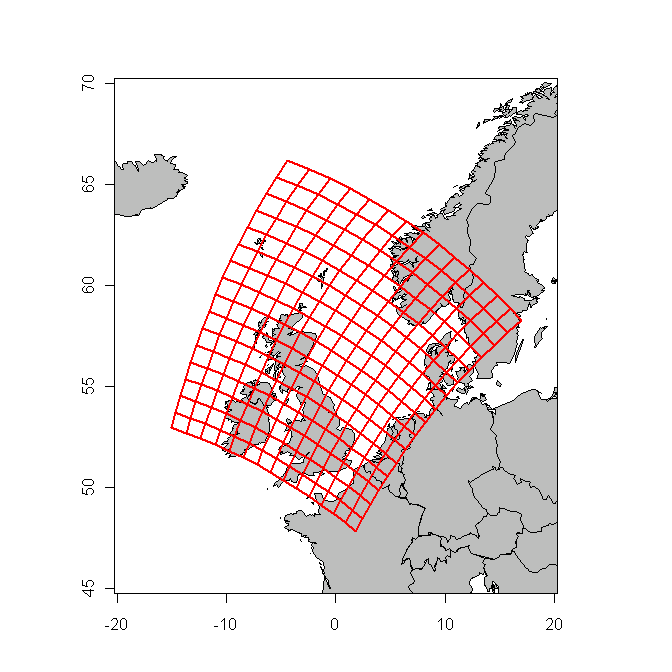
\includegraphics[width=100mm]{figures/NORWECOM_mesh.png}
 \caption{\label{fig:NORWECOM_grid}The NORWECOM mesh plotted on a standard longitude-latitude map. Each square plotted here  corresponds to 10x10 cells.}
\end{figure}

\begin{figure}[t]
 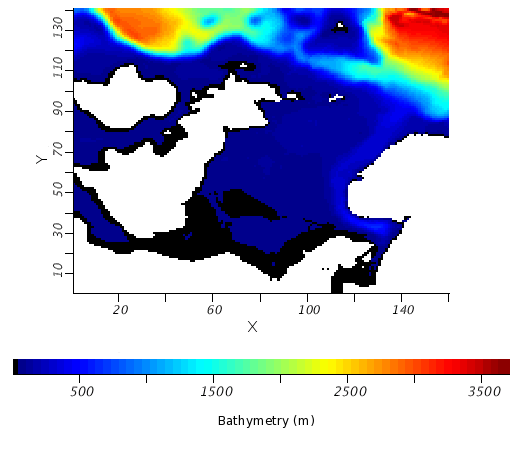
\includegraphics[width=100mm]{figures/NORWECOM_bath.png}
 \centering
 \caption{\label{fig:NORWECOM_topo}The NORWECOM bathymetry plotted using the internal grid \textit{i.e.} the $x$ and $y$ axes.}
\end{figure}

The grid is an ``Arakawa C'' grid (Figure \ref{fig:Arakawa_C}) \textit{i.e.} the tracer properties (temperature, salinity, turbulent diffusivity) are centered in the middle of a cell, whilst the $u$ velocity is located at the centre of the left hand face of the cell and the $v$ velocity is located at the centre of the bottom (``south'') face. The vertical velocity and the vertical diffusivity are measured in the centre of the upper face. The centre of the ($i$th, $j$th) cell is at ($i$-0.5,$j$-0.5): the bottom-left hand corner of the bottom left hand cell therefore has the coordinates (0,0).

\begin{figure}[t]
 \centering
 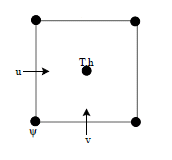
\includegraphics[width=30mm]{figures/Arakawa_C_grid.png}
 \caption{ \label{fig:Arakawa_C}The top view of an Arakawa C grid cell showing where the key parameters are measured: $u$ and $v$ are the velocities and $T$ are the tracer properties \textit{e.g.} temperature, salinity}
\end{figure}

\section{Coordinate Transforms}
The follow relationships can be used to shift between the native grid units, \textit{x}, and \textit{y} to the more familar geographic coordinate system, longitude $\lambda$ and latitude $\phi$. In the oceanography provider, these are implemented by directly ``including'' the corresponding files from the NORWECOM model, \texttt{spr2gr.f} and \texttt{gr2sph.f}. Both $\lambda$ and $\phi$ are expressed here in radians.

\subsection{NORWECOM to Spherical}
\begin{equation}\label{eq:gr2sph}
\begin{aligned}
 d &= \sqrt{DX^2\left(x-x_p\right)^2 + DY^2\left(y-y_p\right)^2} \\
 \lambda &= \alpha + \tan^{-1}\left(\frac{-DX\left(x-x_p\right)}{DY\left(y-y_p\right)}\right) \\
 \phi &= \frac{\pi}{2} - 2\tan^{-1}\left(\frac{d}{R_e\left(1+\sin\phi_0\right)}\right) 
\end{aligned}\end{equation} 

\subsection{Spherical to NORWECOM}
\begin{equation}\label{eq:sph2gr}\begin{aligned}
r &=  R_e\left(1+\sin\phi_0\right)\frac{\cos\phi}{1+\sin\phi}  \\
x &= x_p + \frac{r}{DX} \sin\left(\lambda-\alpha\right) \\
y &= y_p - \frac{r}{DY} \cos\left(\lambda-\alpha\right) 
\end{aligned}\end{equation} 

\subsection{Vertical coordinates}
The vertical layers of the NORWECOM grid are terrain following $\sigma$ coordinates. The transformation between $\sigma$ and depth below the surface, $d$, is
\begin{equation}
  \sigma = \frac{d}{H}
\end{equation} 
where $H$ is the total depth of the water column at the particular point in question. The NORWECOM data set does not include any sea-surface height data, and thus it is not necessary to correct for this factor. $\sigma$ is thus 0 at the surface and 1 at the bottom.


\subsection{Parameters}
The NORWECOM grid is designed to be generic, and can be adapted to many different situations, depending on the specific parameters employed. The details of the North Sea implementation are given below in Table \ref{tbl:NORWECOM_params}.
\begin{table}[h]
	\caption{Grid parameters for the NORWECOM North Sea grid. Note that the angular parameters $\phi_0$ and $\alpha$ are specified in degrees (rather than radians) for convenience.} 
	\centering
	\begin{tabular}{c l l l}
	\hline\hline 
	& Description & Value & Units\\ 
	\hline % inserts single horizontal line
        $DX$ & Average grid spacing in the \textit{x} direction & 10 & km \\
        $DY$ & Average grid spacing in the \textit{y} direction & 10 & km \\
        $x_p$ & $x$ grid coordinate of the North Pole &  382& - \\
        $y_p$ & $y$ grid coordinate of the North Pole & 256& - \\
        $R_e$ & Average radius of the earth & 6370 & km \\
        $\phi_0$ & Latitude of ``true'' length & 60 & deg N\\
        $\alpha$ & Longitude of meridian parallel to the $y$ axis & 58 & deg E\\
	\hline 
	\end{tabular}
	\label{tbl:NORWECOM_params} % is used to refer this table in the text
\end{table}

\section{Coordinate rotations}
The velocities in the NORWECOM database are given as the component velocities parallel to the $x$ and $y$ axes. However, IBMlib requires that they are given as the zonal and meridonal velocities \textit{i.e.} parallel to the latitude and longitude axes. It is therefore necessary to reproject the original $u$ and $v$ velocities accordingly. The matter is further complicated by the fact that the $x$ and $y$ axes are not orthogonal in the spherical coordinate system. Furthermore, any such rotation must take place in such a manner that the length of the vector is maintained \textit{i.e.} the coordinate system is rotated, rather than the vector itself. The approach taken is based on deriving the transformation matrix, $\mathbf{A}$, that describes the relationship between the components in the two different coordinate systems. Given a vector $\vec C$ with components $C_x$ and $C_x$ parallel to the $x$ and $y$ axes, the corresponding components parallel to the $\lambda$ and $\phi$ axes, $C_\lambda$ and $C_\phi$ can be calculated by applying the transformation matrix accordingly:
\begin{equation}\label{eq:transformation_relation}
   \left[\begin{matrix}
    C_\lambda \\ C_\phi
   \end{matrix}\right]
  = \mathbf{A}
   \left[\begin{matrix}
    C_x \\ C_y
   \end{matrix}\right]
\end{equation} 
For simplicity, we have neglected the vertical $z$ dimension, as the vertical axes for both coordinate system are co-incident. 

\subsection{Transformation Matrix}
The orientation of small (linear) deviations about the origin can be determined by considering the total derivatives of $\lambda$ and $\phi$:
\begin{equation}\label{eq:total_derivs}\begin{aligned}
  \operatorname d \lambda &= \frac{\partial \lambda}{\partial x} \operatorname d x + \frac{\partial \lambda}{\partial y} \operatorname d y  \\
  \operatorname d \phi &= \frac{\partial \phi}{\partial x} \operatorname d x + \frac{\partial \phi}{\partial y} \operatorname d y
\end{aligned}\end{equation} 
Equation \eqref{eq:total_derivs} can be rewritten in matrix formulation

\begin{equation}\label{eq:jacobian}\begin{aligned}
 \left[\begin{matrix}
  \operatorname d \lambda \\ \operatorname d \phi 
  \end{matrix}\right]
&= \mathbf{J}  \left[\begin{matrix}
  \operatorname dx  \\  \operatorname dy  
  \end{matrix}\right] \\
\end{aligned}\end{equation}
where $\mathbf{J}$ is the Jacobian matrix:
\begin{equation}\label{eq:jacobian_defn}
\mathbf{J}=\left[\begin{matrix}
   \frac {\partial \lambda}{\partial x}
& \frac {\partial \lambda}{\partial y}
\\  \frac {\partial \phi}{\partial x}
&  \frac {\partial \phi}{\partial y}
\end{matrix}\right]
=\left[\begin{matrix}J_{11} & J_{12} \\ J_{21} & J_{22}  \end{matrix}\right]  
\end{equation}
 
We can use Equation \eqref{eq:jacobian} to deduce the terms of the transformation matrix, $\mathbf A$ by constructing unit vectors parallel to the $x$ and $y$ axes. Consider first an arbitrary change $\Delta x$ in the $x$ direction. The resultant vector,  $\vec{r}$, in $\lambda$ and $\phi$ coordinates is thus
\begin{equation}\begin{aligned}
%Top line---------
 \vec{r} &= \left[\begin{matrix}
  \operatorname d \lambda \\ \operatorname d \phi 
  \end{matrix}\right]
  = \mathbf{J}
  \left[\begin{matrix} \Delta x \\  0 \end{matrix}\right] \\
%Second line---------
&=J_{11}\Delta x \vec e_\lambda + J_{21} \Delta x \vec e_\phi
\end{aligned}
\end{equation}
where $\vec e_\lambda$ and $\vec e_\phi$ are the unit vectors parallel to the $\lambda$ and $\phi$ axes respectively.

The slope of this vector, $m_r$ is given by
\begin{equation}\label{eq:r_slope}
 m_r = \frac{\partial \phi}{\partial \lambda} = \frac{J_{21}}{J_{11}}
\end{equation}

Now let us reconsider the definition of the transformation matrix, $\mathbf{A}$ (Equation \eqref{eq:transformation_relation}) in the same situation for a vector $\vec C$ of length $C_x$ oriented along the $x$ axis:
\begin{equation}\begin{aligned}\label{}
   \vec C = \left[\begin{matrix}
    C_\lambda \\ C_\phi
   \end{matrix}\right]
  &= \mathbf{A}
   \left[\begin{matrix}
    C_x \\ 0
   \end{matrix}\right] 
   = 
   \left[\begin{matrix}
     a_{11} & a_{12} \\ a_{21} & a_{22}
   \end{matrix}\right] 
   \left[\begin{matrix}
    C_x \\ 0
   \end{matrix}\right] 
\\ &= a_{11} C_x \vec e_\lambda + a_{21} C_x \vec e_\phi
\end{aligned}\end{equation}
where $a_{11}$, $a_{12}$... are the individual elements of $\mathbf{A}$. The slope of this vector $m_C$ is given by
\begin{equation}\label{eq:C_slope}
  m_C = \frac{\partial \phi}{\partial \lambda} = \frac{a_{21}}{a_{11}}
\end{equation}
Noting that the $\lambda$ and $\phi$ axes are orthogonal, we can calculate the magnitude of the vector from pythagoras:
\begin{equation*}\begin{aligned}
   \| \vec C\| = \sqrt{{a_{11}}^2 {C_x}^2 + {a_{21}}^2 {C_x}^2}
\end{aligned}\end{equation*} 
However, we know that length of $\vec C$ is $C_x$ and thus can simplify the expression to give:
\begin{equation}\begin{aligned}\label{eq:C_pythag}
   1  = \sqrt{{a_{11}}^2  + {a_{21}}^2 }
\end{aligned}\end{equation} 
Equation \eqref{eq:C_pythag} provides a relationship between two of the terms in the transformation matrix. Equating equations \eqref{eq:r_slope} and \eqref{eq:C_slope} lets us define a further relationship between the componets of the (known) Jacobian and (unknown) transformation matrices:
\begin{equation}\label{eq:C_J_relationship}
  \frac{a_{21}}{a_{11}} = \frac{J_{21}}{J_{11}}
\end{equation}
Thus, combining \eqref{eq:C_pythag} and \eqref{eq:C_J_relationship} and solving gives:
\begin{subequations}\label{eq:transform_dx}\begin{align}
 a_{11} &= \frac{J_{11}}{\sqrt{{J_{11}}^2+{J_{21}}^2}} \\
 a_{21} &= \frac{J_{21}}{\sqrt{{J_{11}}^2+{J_{21}}^2}}
\end{align}\end{subequations}

This process gives us the expressions for two of the terms in the transformation matrix. The other two terms can be dervied by repeating the process for an arbitrary step in the $y$ direction to yield:
\begin{subequations}\label{eq:transform_dy}\begin{align}
 a_{12} &= \frac{J_{12}}{\sqrt{{J_{12}}^2+{J_{22}}^2}} \\
 a_{22} &= \frac{J_{22}}{\sqrt{{J_{12}}^2+{J_{22}}^2}}
\end{align}\end{subequations}
Combining the two sets of results, \eqref{eq:transform_dx} and \eqref{eq:transform_dy}, we can write the final expression for the transformation matrix, $\mathbf{A}$ as a version of the Jacobian matrix, $\mathbf{J}$ where the columns are unit vectors:
\begin{equation}
  \mathbf{A} = \mathbf{J}
   \left[\begin{matrix}
      \frac{1}{\sqrt{{J_{11}}^2+{J_{21}}^2}}
&     0 \\   0 &
     \frac{1}{\sqrt{{J_{12}}^2+{J_{22}}^2}}
                     \end{matrix}\right]
\end{equation}


\subsection{Jacobian Matrix Formulae}
The individual elements of the Jacobian Matrix can be determined by evaluating the appropriate partial derivatives of Equation \eqref{eq:gr2sph} to give the following system of equations:

\begin{subequations}\begin{align}
d &= \sqrt{{DX}^2{\left(x-x_p\right)}^2 + {DY}^2{\left(y-y_p\right)}^2}\\
g &= R_e\left(1+\sin\phi_0\right) \\
J_{11} = \frac {\partial \lambda}{\partial x} 
       &= \frac{-DXDY}{d^2}\left(y-y_p\right)\\
J_{12} = \frac {\partial \lambda}{\partial y}
       &= \frac{DXDY}{d^2}\left(x-x_p\right)\\
J_{21} = \frac {\partial \phi}  {\partial x}
       &= \frac{-2}{gd\left(1+\frac{d^2}{g^2}\right)} \left(x-x_p\right){DX}^2\\
J_{22} =  \frac {\partial \phi}{\partial y}
       &= \frac{-2}{gd\left(1+\frac{d^2}{g^2}\right)} \left(y-y_p\right){DY}^2
\end{align}\end{subequations}

\subsection{Turbulence derivatives}
IBMlib requires the derivative of the turbulent diffusivities as part of its input. These derivatives need to be in units of m²/s/m with the derivatives oriented in directions parallel to the latitude and longitude vectors. However, it is more convenient to estimate the derivatives directly in the native NORWECOM grid ($e.g.$ using the built in regular grid interpolators in IBMlib) - unfortunately, this results in derivatives in units of m²/s/grid, oriented parallel to the grid axes. Here we detail the transformation between the two sets of derivatives.

Consider first the derivatives with respect to grid units, $\frac{dD}{dx}$ and $\frac{dD}{dy}$. Applying the chain rule, we can write
\begin{subequations}\begin{align}
\frac{dD}{dx} = \frac {\partial D}{\partial s}\frac {\partial s}{\partial x}  +
       \frac {\partial D}{\partial t}\frac {\partial t}{\partial x} \\
\frac{dD}{dy} = \frac {\partial D}{\partial s}\frac {\partial s}{\partial y}  +
       \frac {\partial D}{\partial t}\frac {\partial t}{\partial y}
\end{align}\end{subequations}
where $s$ and $t$ are the distances (in metres) on the surface of the earth oriented parallel to the longitude and latitudinal axes. We can write this expression in matrix notation
\begin{equation}
\left[\begin{matrix} 
	  \frac{dD}{dx} \\ 
	  \frac{dD}{dy} 
	  \end{matrix}\right] 
= \left[\begin{matrix} 
         \frac {\partial s}{\partial x}  & \frac {\partial t}{\partial x} \\
         \frac {\partial s}{\partial y}  & \frac {\partial t}{\partial y} \\
        \end{matrix}\right]
 \left[\begin{matrix} 
         \frac {\partial D}{\partial s}  \\
         \frac {\partial D}{\partial t}  
        \end{matrix}\right]
\end{equation}
We can expand the 2x2 matrix using the chain rule again to express the derivatives in terms of the longitude $\lambda$ and latitude $\phi$.
\begin{equation}
\left[\begin{matrix} 
	  \frac{dD}{dx} \\ 
	  \frac{dD}{dy} 
	  \end{matrix}\right] 
= \left[\begin{matrix} 
         \frac {\partial \lambda}{\partial x}  & \frac {\partial \phi}{\partial x} \\
         \frac {\partial \lambda}{\partial y}  & \frac {\partial \phi}{\partial y} \\
        \end{matrix}\right]
 \left[\begin{matrix} 
         \frac {\partial s}{\partial \lambda}  & \frac {\partial t}{\partial \lambda} \\
         \frac {\partial s}{\partial \phi}  & \frac {\partial t}{\partial \phi} \\
        \end{matrix}\right]
 \left[\begin{matrix} 
         \frac {\partial D}{\partial s}  \\
         \frac {\partial D}{\partial t}  
        \end{matrix}\right]
\end{equation}

We note that the first 2x2 matrix on the right hand side is simply the transpose of the jacobian $\mathbf{J}$ above (Equation \eqref{eq:jacobian_defn}). Solving for  $\frac{dD}{ds}$ and $\frac{dD}{dt}$ thus gives
\begin{equation}
\left[\begin{matrix} 
         \frac {\partial D}{\partial s}  \\
         \frac {\partial D}{\partial t}  
        \end{matrix}\right]
= \left[\begin{matrix} 
         \frac {\partial s}{\partial \lambda}  & \frac {\partial t}{\partial \lambda} \\
         \frac {\partial s}{\partial \phi}  & \frac {\partial t}{\partial \phi} \\
        \end{matrix}\right]^{-1}
\mathbf{J}^{-T}
\left[\begin{matrix} 
	  \frac{dD}{dx} \\ 
	  \frac{dD}{dy} 
	  \end{matrix}\right] 
\end{equation}
The relationship between $s$, $t$, $\lambda$ and $\phi$ is given from simple spherical geometry describing the distances on the surface of a sphere of radius $R$.
\begin{subequations}\begin{align}
s&=R\lambda\cos\phi \\t&=R\phi
\end{align}\end{subequations}
Evaluating the remaining derivatives, and inverting the matrix gives the desired expression.
\begin{equation}
\left[\begin{matrix} 
         \frac {\partial D}{\partial s}  \\
         \frac {\partial D}{\partial t}  
        \end{matrix}\right]
= \left[\begin{matrix} 
         \frac {1}{R \cos \phi}  & 0 \\
         \frac {\lambda \tan \phi}{R}  & \frac {1}{R}
        \end{matrix}\right]
\mathbf{J}^{-T}
\left[\begin{matrix} 
	  \frac{dD}{dx} \\ 
	  \frac{dD}{dy} 
	  \end{matrix}\right] 
\end{equation}





\section{Configuration}
The NORWECOM oceanography provider requires two variables to be supplied in the IBMlib controlfile.\begin{itemize}
 \item \texttt{hydroDBpath} species the directory containing the NORWECOM data files. 
 \item \texttt{bath\_file} specifies a selected NORWECOM netcdf file that contains the bathymetry to be used. Generally, each NORWECOM file contains the bathymetry data - however, for consistency and simplicity, it is easier to choose just a single file as being representative of the bathymetry: this value is then used throughout the entire IBMlib run.
\end{itemize}


\section{Major Revisions}
The following list summarises the major revisions of the NORWECOM pbi
\begin{itemize}
 \item \texttt{r233} Initial version merged to trunk, with all features working. Coastline intersection needs generalisation to a generic grid. Interpolation around the coastlines is piecewise and could be improved.
\end{itemize}

\end{document}
